



\title{Solana: Una nuova architettura per una blockchain ad alte prestazioni  v0.8.14 }

\author{
        Anatoly Yakovenko \\
        anatoly@solana.io\\
}
\date{}

\documentclass[12pt]{article}

% \usepackage{draftwatermark}
% \SetWatermarkText{Confidential}
% \SetWatermarkScale{5}
% \SetWatermarkColor[gray]{0.95}

\usepackage{graphicx}
\usepackage{bytefield}
\usepackage{makecell}
\usepackage[utf8]{inputenc}


\usepackage[]{hyperref}
\hypersetup{
    pdftitle={Solana:  Una nuova architettura per una blockchain ad alte prestazioni},
    pdfauthor={anatoly@solana.io},
    pdfsubject={blockchain},
    pdfkeywords={blockchain, bitcoin, cryptocurrency},
    bookmarksnumbered=true,
    bookmarksopen=true,
    bookmarksopenlevel=1,
    colorlinks=true,
    pdfstartview=Fit,
    pdfpagemode=UseOutlines,    % this is the option you were lookin for
    pdfpagelayout=TwoPageRight
}

\begin{document}
\maketitle

\textbf{\footnotesize Esonero Legale}\scriptsize
~~Nulla nel presente White Paper è un'offerta di vendita o un modo per indurre all' acquisto di token. Solana pubblica questo White Paper esclusivamente per ricevere feedback e commenti da parte del pubblico. Se e quando Solana metterà in vendita dei token (o un semplice accordo per token futuri), lo farà attraverso documenti di offerta definitivi, tra cui un documento informativo e fattori di rischio. Si prevede che tali documenti definitivi comprenderanno anche una versione aggiornata del White Paper, che potrebbe differire in misura significativa dalla versione attuale. Se e quando Solana farà tale offerta negli Stati Uniti, l'offerta sarà probabilmente disponibile solo per gli investitori accreditati.


Nessun elemento del presente White Paper deve essere trattato o letto come una garanzia o una promessa di come si svilupperanno le attività di Solana  o dell'utilità o del valore dei gettoni o di come essi verranno distribuiti. Il presente White Paper delinea i piani attuali, che potrebbero cambiare a discrezione di Solana e il cui successo dipenderà da molti fattori al di fuori del controllo di Solana, tra cui i fattori di mercato e i fattori nel settore dei dati e della industria delle cryptovalute. Qualsiasi dichiarazione su eventi futuri si basa esclusivamente sull'analisi delle questioni descritte nel presente White Paper effettuata da Solana. Tale analisi potrebbe rivelarsi errata.


\begin{abstract}\label{Astratto}
Il presente documento propone una nuova architettura blockchain basata sulla Proof of History (PoH) - una prova per verificare l'ordine e il passaggio del tempo tra gli eventi. PoH è usato per codificare il passaggio sicuro del tempo in un libro mastro - una struttura di dati solo append. Se utilizzato insieme a un algoritmo di consenso come il Proof of Work (PoW) o il Proof of Stake (PoS), il PoH può ridurre l'overhead in un di messaggistica in una macchina a stato replicato Byzantine Fault Tolerant, con tempi di finalizzazione inferiori ai secondi. Questo articolo propone anche due algoritmi che sfruttano le proprietà di conservazione del tempo del registro PoH - un algoritmo PoS che può recuperare da partizioni di qualsiasi dimensione e un efficiente streaming Proof of Replication (PoRep). La combinazione di PoRep e PoH fornisce una difesa contro la falsificazione del libro mastro per quanto riguarda il tempo (ordinamento) e la conservazione. Il protocollo viene analizzato su una rete da $1$~gbps e questo articolo mostra che con l'hardware odierno è possibile effettuare transazioni fino a $710$k al secondo.

\end{abstract}


\section{Introduzione}\normalsize
Blockchain è l'implementazione di una macchina a stato replicato con tolleranza ai guasti. Le blockchain attualmente disponibili al pubblico non si basano sul tempo, o fanno un'ipotesi debole sulle capacità del partecipante di mantenere il tempo~\cite{tendermint,hashgraph}. Ogni nodo della rete di solito si basa sul proprio orologio locale senza che gli altri partecipanti ne siano a conoscenza. La mancanza di una fonte di tempo affidabile significa che quando un messaggio viene utilizzato per accettare o rifiutare un messaggio, non vi è alcuna garanzia che ogni altro partecipante alla rete effettuerà la stessa scelta. Il PoH qui presentato è stato progettato per creare un registro con un passaggio di tempo verificabile, cioè la durata tra gli eventi e l'ordinazione dei messaggi. Si prevede che ogni nodo della rete potrà contare sul passaggio del tempo registrato nel libro mastro senza doversi fidare di terze parti.

\section{Indice}
Il resto di questo articolo è organizzato come segue. La progettazione generale del sistema è descritta nella Sezione ~\ref{design}. Una descrizione dettagliata della Proof of History è descritta nella Sezione ~\ref{proof_of_history}. Una descrizione dettagliata dell'algoritmo Proof of Stake proposto per la verifica del consenso  è descritta nella sezione~\ref{proof_of_stake}. Una descrizione dettagliata della fast Proof of Replication  è descritta nella Sezione ~\ref{porep}. L'architettura di sistema e i limiti delle prestazioni sono analizzati nella Sezione ~\ref{architettura_di_sistema}. Un motore a contratto intelligente ad alte prestazioni e facile da usare per le GPU è descritto nella Sezione ~\ref{sec:smartcontracts}.

\section{Network Design}\label{design}

\begin{figure}[h]
  \begin{center}
    \centering
    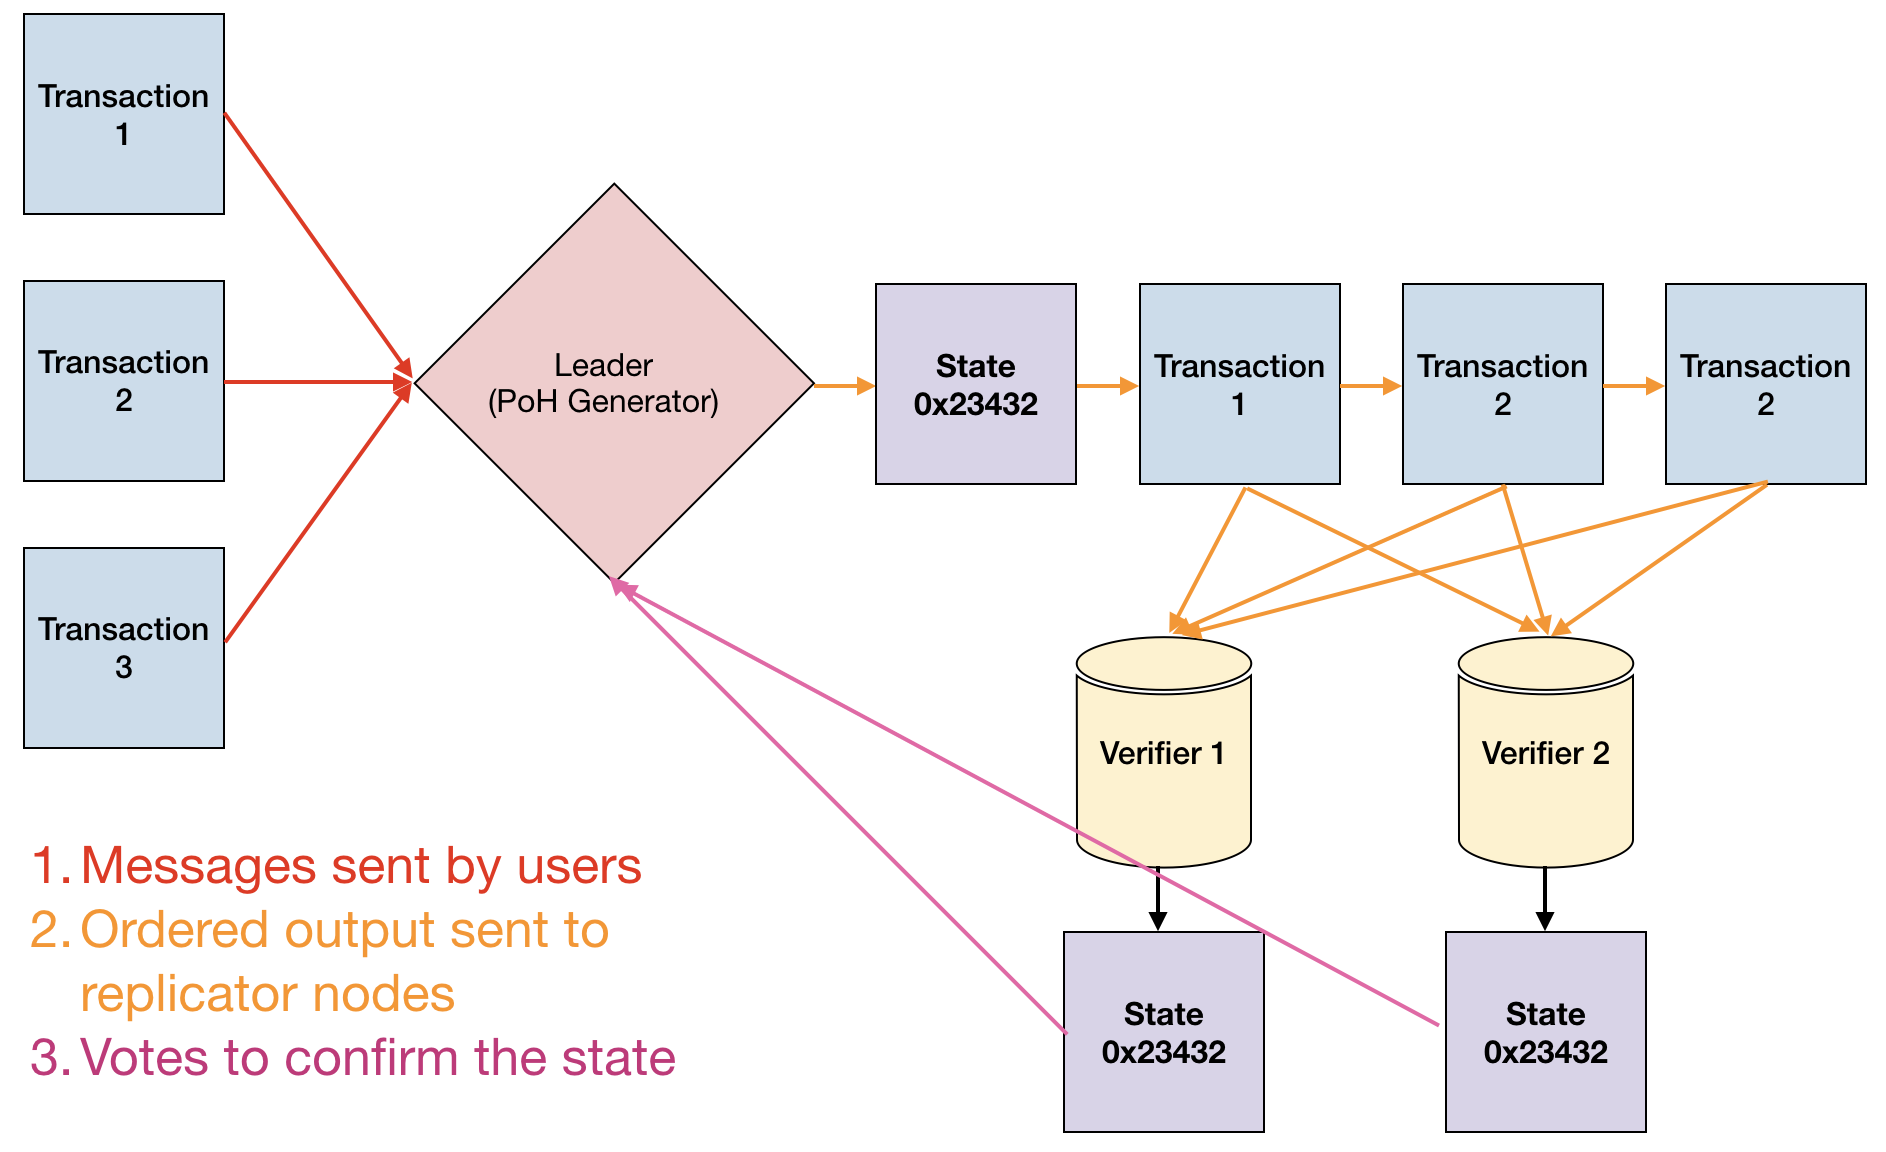
\includegraphics[width=\textwidth]{figures/network_design_001.png}
    \caption[Fig 1]{Transazioni attraverso la rete.\label{fig:design}}
  \end{center}
  \end{figure}

Come mostrato nella Figura~\ref{fig:design}, in qualsiasi momento un nodo di sistema è designato come Leader per generare una sequenza di Proof of History, fornendo alla rete una coerenza di lettura globale e un passaggio del tempo verificabile. Il Leader sequenzia i messaggi degli utenti e li ordina in modo tale che possano essere elaborati in modo efficiente da altri nodi del sistema, massimizzando la produttività. Il Leader esegue le transazioni sullo stato corrente memorizzato nella RAM e pubblica le transazioni e una firma dello stato finale sui nodi di replica chiamati Verificatori. I Verificatori eseguono le stesse operazioni sulle loro copie dello stato e pubblicano le loro firme calcolate dello stato come conferme. Le conferme pubblicate servono come voti per l'algoritmo di consenso.

In uno stato non partizionato, in qualsiasi momento, c'è un Leader nella rete. Ciascun nodo verificatore ha le stesse capacità hardware di un Leader e può essere eletto Leader, questo avviene tramite elezioni basate su PdS. Le elezioni per l'algoritmo di PdS proposto sono trattate in modo approfondito nella Sezione~\ref{subsec:elections}.

Per il di teorema CAP, la Coerenza è quasi sempre scelta rispetto alla Disponibilità in caso di Partizione. Nel caso di una partizione di grandi dimensioni, questo documento propone un meccanismo per ripristinare il controllo della rete da una partizione di qualsiasi dimensione. Questo è trattato in modo approfondito nella Sezione~\ref{availability}.	

\section{Proof of History}\label{proof_of_history}

La Proof of History è una sequenza di calcolo che può fornire un modo per verificare crittograficamente il passaggio del tempo tra due eventi. Utilizza una funzione di sicurezza crittografica scritta in modo che non sia possibile prevedere l'uscita dall'ingresso e che debba essere eseguita completamente per generare l'uscita. La funzione viene eseguita in sequenza su un singolo core, la cui uscita precedente è l'ingresso corrente, registrando periodicamente l'uscita corrente e quante volte è stata richiamata. L'uscita può quindi essere ricalcolata e verificata da computer esterni in parallelo controllando ogni segmento di sequenza su un nucleo separato.

I dati possono essere timestampati in questa sequenza aggiungendo i dati (o un hash di alcuni dati) nello stato della funzione. La registrazione dello stato, dell'indice e dei dati così come sono stati aggiunti alle sequenze fornisce una timestamp in grado di garantire che i dati siano stati creati in un momento precedente alla generazione dell'hash successivo nella sequenza. Questo design supporta anche l'horizontal scaling, in quanto più generatori possono sincronizzarsi tra loro mescolando il loro stato nelle sequenze degli altri. L'horizontal scaling è discusso in modo approfondito nella Sezione~\ref{poh:scale}\\

\subsection{Description}
Il sistema è progettato per funzionare come segue. Con una funzione hash crittografica, il cui output non può essere previsto senza eseguire la funzione (ad esempio \texttt{sha256}, \texttt{ripemd}, ecc.), eseguire la funzione da un valore iniziale casuale e prenderne l'output e passarlo nuovamente come ingresso nella stessa funzione. Registrare il numero di volte che la funzione è stata richiamata e l'uscita ad ogni chiamata. Il valore casuale di partenza scelto potrebbe essere qualsiasi stringa, come la prima pagina del New York Times di quel giorno.
\\\\
\noindent Per esempio: \noindent
\begin{center}
  \begin{tabular}{  l  l  r }
%    \hline
    \multicolumn{3}{c}{Sequenza PoH} \\
    \hline
    Index  & Operation & Output Hash \\ \hline
    $1$ & sha256(\char`\"any random starting value\char`\") & \texttt{hash1}\\ %\hline
    $2$ &  sha256(\texttt{hash1}) & \texttt{hash2}\\ %\hline
    $3$ & sha256(\texttt{hash2}) & \texttt{hash3}\\ %\hline
    \end{tabular}
\end{center}

\noindent Dove \texttt{hashN} rappresenta l'attuale outtup dell'hash.\\

È solo necessario pubblicare un subset degli hashes e degli indici ad un intervallo.\\

\noindent Per esempio:\\\\\noindent
\begin{center}
  \begin{tabular}{ l  l  r }
    \multicolumn{3}{c}{PoH Sequence} \\
    \hline
    Index & Operation & Output Hash \\ \hline
    $1$ & sha256(\char`\"any random starting value\char`\") & \texttt{hash1}\\
    $200$ &  sha256(\texttt{hash199}) & \texttt{hash200}\\
    $300$ & sha256(\texttt{hash299}) & \texttt{hash300} \\
    \end{tabular}
\end{center}

Finché la funzione hash scelta è resistente alle collisioni, questa serie di hash può essere calcolata in sequenza solo da un singolo thread del computer. Questo deriva dal fatto che non c'è modo di prevedere quale sarà il valore hash dell'indice $300$ senza eseguire l'algoritmo a partire dal valore iniziale $300$ volte. Così possiamo dedurre dalla struttura dei dati che del tempo reale è passato tra l'indice $0$ e l'indice $300$.

Nell'esempio in Figura~\ref{fig:poh_seq}, l'hash \texttt{62f51643c1} è stato prodotto contando fino a $510144806912$ e l'hash \texttt{c43d862d88} è stato prodotto contando fino a $510146904064$. Seguendo le proprietà precedentemente discusse dell'algoritmo PoH, possiamo fidarci che sia passato tempo reale tra il conteggio $510144806912$ e il conteggio $510146904064$.

\begin{figure}[h]
  \begin{center}
    \centering
    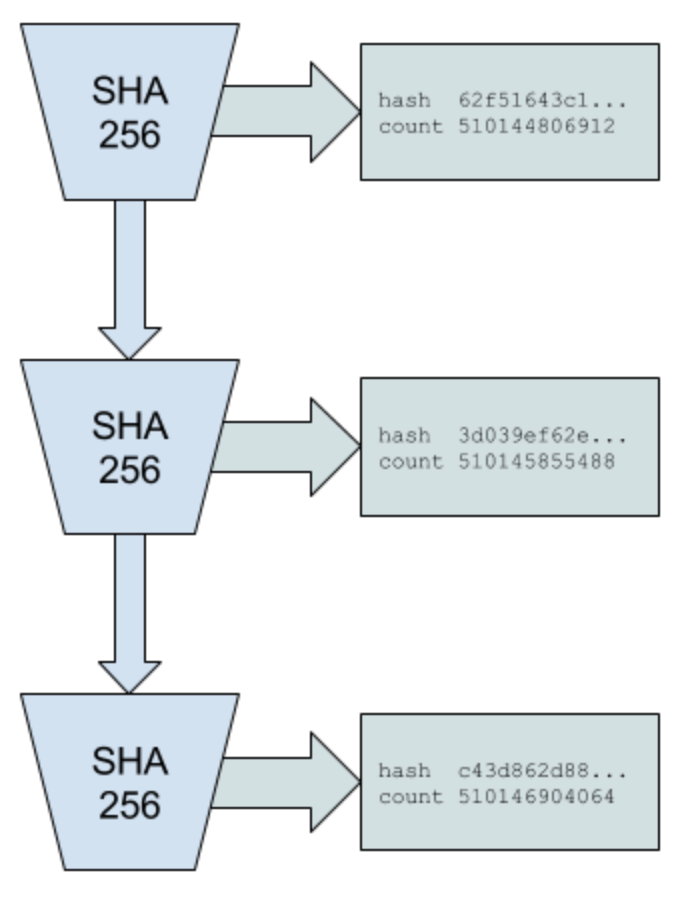
\includegraphics[width=0.5\textwidth]{figures/poh_sequence_001.png}
    \caption[Figure 2]{Sequenza Proof of History\label{fig:poh_seq}}
  \end{center}
  \end{figure}

\subsection{Timestamp for Events}

La sequenza di hash può anche essere usata per registrare che alcuni dati sono stati creati prima che fosse generato un particolare indice hash utilizzando una funzione "combina" per combinare il dato con l'hash corrente nell'indice corrente. I dati possono essere un hash crittograficamente univoco di dati di eventi arbitrari. La funzione combina può essere una semplice aggiunta di dati, o qualsiasi operazione che sia resistente alle collisioni. L'hash successivo generato rappresenta un timestamp dei dati, perché avrebbe potuto essere generato solo dopo l'inserimento di quel dato specifico.\\

\noindent Ad Esempio:\\\\\noindent
\begin{center}
  \begin{tabular}{ l l r }
    \multicolumn{3}{c}{PoH Sequence} \\
    \hline
    Index  & Operation  & Output Hash\\ \hline
    $1$ & sha256(\char`\"any random starting value\char`\") & \texttt{hash1}\\
    $200$ & sha256(\texttt{hash199}) & \texttt{hash200}\\
    $300$ & sha256(\texttt{hash299}) & \texttt{hash300}\\
    \end{tabular}
\end{center}


	\noindent Si verifica qualche evento esterno, come scattare una foto, oppure
	vengono creati dati digitali arbitrari:\\\\\noindent
\begin{center}
  \begin{tabular}{ l l r}
    \multicolumn{3}{c}{PoH Sequence With Data} \\
    \hline
    Index  & Operation & Output Hash\\ \hline
    $1$ & sha256(\char`\"any random starting value\char`\") & \texttt{hash1} \\
    $200$ & sha256(\texttt{hash199}) & \texttt{hash200} \\
    $300$  & sha256(\texttt{hash299}) & \texttt{hash300}\\
    $336$ & sha256(append(\texttt{hash335}, photograph\_sha256)) & \texttt{hash336}\\
    \end{tabular}
\end{center}


\texttt{Hash336} è calcolato a partire dai dati binari allegati di
\texttt{hash335} e il \texttt{sha256} della fotografia. L'indice
e il \texttt{sha256} della fotografia sono registrati come parte del file 
uscito in sequenza. Chiunque verifichi questa sequenza può quindi ricreare
questa modifica alla sequenza. La verifica può ancora essere effettuata in
parallelo ed è discusso nella Sezione ~\ref{poh:verify}

Poiché il processo iniziale è ancora sequenziale, possiamo dire che le cose inserite nella sequenza devono essersi verificate prima che il futuro valore fosse calcolato.

\begin{center}
  \begin{table}
  \begin{tabular}{l l r}
    \multicolumn{3}{c}{POH Sequence} \\ \hline
    Index & Operation & Output Hash \\ \hline
    $1$ & sha256(\char`\"any random starting value\char`\") & \texttt{hash1} \\
    $200$ & sha256(hash199) & \texttt{hash200} \\
    $300$ & sha256(hash299) & \texttt{hash300} \\
    $336$ & sha256(append(hash335, photograph1\_sha256)) & \texttt{hash336}\\
    $400$ & sha256(hash399) & \texttt{hash400} \\
    $500$ & sha256(hash499) & \texttt{hash500}\\
    $600$ & sha256(append(hash599, photograph2\_sha256)) & \texttt{hash600}\\
    $700$ & sha256(hash699) & \texttt{hash700}\\
    \end{tabular}
    \caption[Tabella 1]{Sequenza PoH con 2 eventi\label{table:multievent}}
    \end{table}
\end{center}

Nella sequenza rappresentata da Table~\ref{table:multievent}, \texttt{photograph2} è stato creato prima di \texttt{hash600}, e
\texttt{foto1} è stato creato prima di \texttt{hash336}. L'inserimento dei dati nella sequenza degli hash comporta la modifica di tutti i valori successivi della sequenza. Finché la funzione hash utilizzata è resistente alle collisioni e i dati sono stati aggiunti, dovrebbe essere impossibile calcolare in anticipo le sequenze future sulla base di una conoscenza preliminare dei dati che saranno integrati nella sequenza.\\

I dati che vengono mixati nella sequenza possono essere i dati grezzi stessi, o semplicemente un hash dei dati con i metadati di accompagnamento.\\

\begin{figure}[h]
  \begin{center}
    \centering
    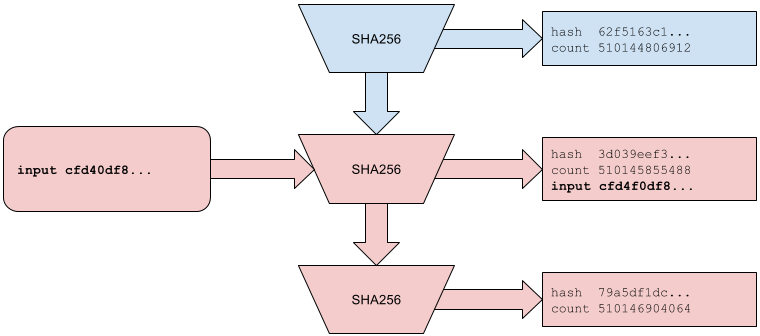
\includegraphics[width=0.9\textwidth]{figures/fig_3.png}
    \caption[Fig 3]{Inserimento dei dati nella Proof of History\label{fig:poh_insert}}
  \end{center}
  \end{figure}

  Nell'esempio in Figura~\ref{fig:poh_insert}, l'input \texttt{cfd40df8\ldots} è stato inserito nella sequenza della Proof of History. Il conteggio a cui è stato inserito è $510145855488$ e lo stato in cui è stato inserito è \texttt{3d039eef3}. Tutti gli hash generati in futuro vengono modificati da questo cambiamento nella sequenza, questo cambiamento è indicato dal cambiamento di colore nella figura.\\

Ogni nodo che osservi questa sequenza può determinare l'ordine in cui sono stati inseriti tutti gli eventi e stimare il tempo reale tra gli inserimenti.

\subsection{Verifica}\label{poh:verify}
La correttezza della sequenza può essere verificata da un computer multicore in un tempo significativamente inferiore a quello necessario per generarla.\\

\noindent Ad esempio: \\\noindent

\begin{center}

\begin{tabular}{l l r}
    \multicolumn{3}{c}{Core 1} \\ \hline
    Index & Data & Output Hash \\ \hline
    $200$ & sha256(\texttt{hash199}) & \texttt{hash200} \\
    $300$ & sha256(\texttt{hash299}) & \texttt{hash300}\\
    \end{tabular}\\

  \begin{tabular}{l l r}
    \multicolumn{3}{c}{Core 2} \\
    \hline
    Index & Data & Output Hash \\ \hline
    $300$ & sha256(\texttt{hash299}) & \texttt{hash300} \\
    $400$ & sha256(\texttt{hash399}) & \texttt{hash400}\\
    \end{tabular}

\end{center}


Dato un certo numero di core, come quelli di una moderna GPU con $4000$ core , il verificatore può dividere la sequenza di hash e i loro indici in $4000$ sezioni  e in parallelo assicurarsi che ogni sezione sia corretta dall'hash iniziale all'ultimo hash nella sezione. Se il tempo previsto per produrre la sequenza è:\\


\[
\frac{\textrm{Numero totale degli hash}}{\textrm{Hash al secondo per 1 core}}
\]

\noindent Il tempo previsto per verificare che la sequenza sia corretta è:\\

\[
\frac{\textrm{Numero totale degli hash}}{\textrm{(Hash al secondo per core * Numero dei core disponibili alla verifica)}}
\]

\begin{figure}
  \begin{center}
    \centering
    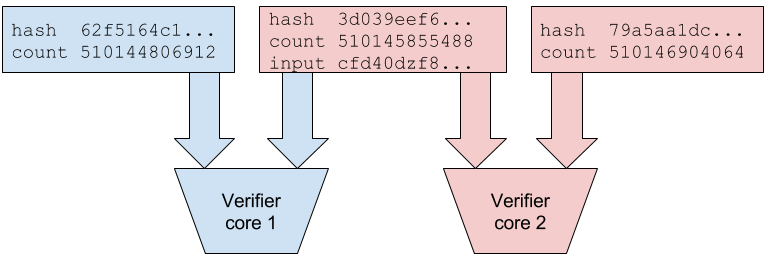
\includegraphics[width=0.9\textwidth]{figures/fig_4.png}
    \caption[Figure 4]{Verifica usando più core\label{fig:poh_verify}}
  \end{center}
  \end{figure}

Nell'esempio in Figura~\ref{fig:poh_verify}, ogni nucleo è in grado di verificare ogni sezione della sequenza in parallelo. Poiché tutte le stringhe di ingresso vengono registrate nell'uscita, con il contatore e lo stato in cui sono aggiunte, i verificatori possono replicare ogni striscia in parallelo. Gli hash di colore rosso indicano che la sequenza è stata modificata mediante l'inserimento di dati.

\subsection{Scaling Orizzontale}\label{poh:scale}
È possibile sincronizzare più generatori Proof of History mescolando lo stato di sequenza da un generatore all'altro e ottenendo così lo scaling orizzontale del generatore Proof of History. Questo scaling è fatto senza sharding. È necessaria l'uscita di entrambi i generatori  per ricostruire l'intero ordine degli eventi nel sistema.

\begin{center}
  \begin{tabular}{|l c r|}

  \hline
    \multicolumn{3}{|c|}{PoH Generator A} \\
  %  \hline
    Index & Hash & Data \\ \hline
    $1$ & \texttt{hash1a} & \\
    $2$ & \texttt{hash2a} & \texttt{hash1b} \\
    $3$ & \texttt{hash3a} & \\
    $4$ & \texttt{hash4a} & \\
    \hline
    \end{tabular}
  \begin{tabular}{| l  c  r |}
  \hline
    \multicolumn{3}{|c|}{PoH Generator B} \\
%    \hline
    Index & Hash & Data \\ \hline
    $1$ & \texttt{hash1b} & \\
    $2$ & \texttt{hash2b} & \texttt{hash1a} \\
    $3$ & \texttt{hash3b} & \\
    $4$ & \texttt{hash4b} & \\
    \hline
    \end{tabular}
\end{center}

Dati i generatori A e B, A riceve un pacchetto di dati da B (hash1b), che contiene l'ultimo stato dal generatore B, e l'ultimo stato dal generatore B osservato dal generatore A. L'hash di stato successivo nel generatore A dipende quindi dallo stato dal generatore B, quindi possiamo dedurre che hash1b è successo qualche tempo prima di hash3a. Questa proprietà è transitiva, quindi se tre generatori sono sincronizzati tramite un unico generatore comune \(A \leftrightarrow B \leftrightarrow C\), possiamo tracciare la dipendenza tra A e C anche se non sono stati sincronizzati direttamente.

Sincronizzando periodicamente i generatori, ogni generatore può quindi gestire una parte del traffico esterno, in modo che il sistema complessivo possa gestire una maggiore quantità di eventi da monitorare che dipende dall'accuratezza del tempo reale, a causa di latenze di rete tra i generatori. Un ordine globale può ancora essere raggiunto selezionando una funzione deterministica per ordinare qualsiasi evento che si trovi all'interno della finestra di sincronizzazione, come ad esempio il valore dell'hash stesso.


\begin{figure}
  \begin{center}
    \centering
    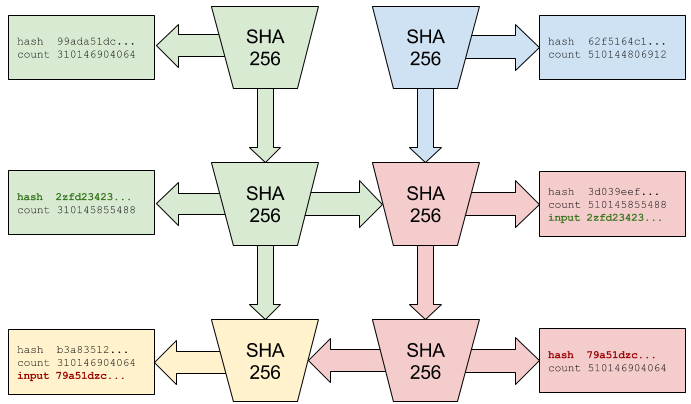
\includegraphics[width=0.9\textwidth]{figures/fig_5.png}
    \caption[Fig 5]{Sincronizzazione di due generatori\label{fig:poh_scale}}
  \end{center}
  \end{figure}

Nella Figura~\ref{fig:poh_scale}, i due generatori inseriscono lo stato di uscita dell'altro e registrano l'operazione. Il cambio di colore indica che i dati del peer hanno modificato la sequenza.  Le hash generate che vengono mixate in ciascun flusso sono evidenziate in grassetto. 

La sincronizzazione ha proprietà transitiva. \(A \leftrightarrow B \leftrightarrow C\). Esiste un ordine dimostrabile di eventi tra A e C attraverso B.

%%It is worth noting that the theoretical $710$k tx/s on a $1$~gb network based on the PoH design does not account for additional capacity offered through  horizontal scaling.
Questo tipo di scaling è limitato dalla Disponibilità. Connessioni da $10 \times 1$~gbps con disponibilità di 0,999 avrebbero disponibilità \(0,999^{10} = 0,99 \).

\subsection{Consistenza}
Gli utenti devono essere in grado di imporre la coerenza della sequenza generata e renderla resistente agli attacchi inserendo l'ultimo output osservato della sequenza che considerano valida nel loro input.\\

\begin{center}
  \begin{tabular}{ | l c r |}
    \hline
    \multicolumn{3}{|c|}{PoH Sequence A} \\
    Index & Data & Output Hash  \\ \hline
    $10$ & & \texttt{hash10a} \\
    $20$ & Event1 & \texttt{hash20a} \\
    $30$ & Event2 & \texttt{hash30a} \\
    $40$ & Event3 & \texttt{hash40a} \\
    \hline
    \end{tabular}
  \begin{tabular}{ | l c r |}
    \hline
    \multicolumn{3}{|c|}{PoH Hidden Sequence B} \\
    Index & Data & Output Hash \\ \hline
    $10$ & & \texttt{hash10b}\\
    $20$ & Event3 & \texttt{hash20b}  \\
    $30$ & Event2 & \texttt{hash30b} \\
    $40$ & Event1 & \texttt{hash40b} \\
    \hline
    \end{tabular}
\end{center}

Se un generatore di PoH dannoso ha accesso a tutti gli eventi contemporaneamente è in grado di generare una sequenza nascosta più rapida oppure può produrre una seconda sequenza nascosta con gli eventi in ordine inverso.\\

Per prevenire questo attacco, ogni Evento generato dal client dovrebbe contenere in sé l'ultimo hash che il client ha osservato da quella che considera una sequenza valida. Quindi, quando un client crea i dati "Event1", dovrebbe aggiungere l'ultimo hash che ha osservato.\\

\begin{center}
  \begin{tabular}{  l  c l}

    \multicolumn{3}{c}{PoH Sequence A} \\
    \hline
    Index  & Data & Output Hash  \\ \hline
    $10$ & & \texttt{hash10a} \\
    $20$ & Event1 = append(event1 data, \texttt{hash10a}) & \texttt{hash20a}  \\
    $30$ & Event2 = append(event2 data, \texttt{hash20a}) & \texttt{hash30a} \\
    $40$ &  Event3 = append(event3 data, \texttt{hash30a}) & \texttt{hash40a} \\
    \end{tabular}
\end{center}

Quando la sequenza viene pubblicata, Event3 fa riferimento a hash30a, e se non è nella sequenza precedente a questo Evento, gli utenti della sequenza sanno che è una sequenza non valida. L'attacco parziale di riordino sarebbe quindi limitato al numero di hash prodotti dal momento in cui il client ha osservato un evento a quando l'evento è stato inserito. I client dovrebbero quindi essere in grado di scrivere software senza presumere che l'ordine sia corretto per il breve periodo di hash tra l'ultimo hash osservato e quello inserito.

Per evitare che un generatore di PoH dannoso riscriva le hash dell'evento del client, i client possono inviare una firma dei dati dell'evento e l'ultimo hash osservato al posto dei soli dati.\\
\begin{center}
  \begin{tabular}{  l  l  r }
    \multicolumn{3}{c}{PoH Sequence A} \\
    \hline
    Index & Data & Output Hash \\ \hline
    $10$ & & hash10a  \\
    $20$ & \makecell{Event1 = sign(append(event1 data, hash10a), \\Client Private Key)} & hash20a\\
    $30$ & \makecell{Event2 = sign(append(event2 data, hash20a), \\Client Private Key)} & hash30a \\
    $40$ & \makecell{Event3 = sign(append(event3 data, hash30a), \\Client Private Key)} & hash40a \\

    \end{tabular}
\end{center}

La verifica di questi dati richiede una verifica della firma e una ricerca dell'hash nella sequenza di hash precedenti a questo..\\
\noindent Verifica:\\

\noindent\texttt{(Signature, PublicKey, hash30a, event3 data) = Event3} \\
\texttt{Verify(Signature, PublicKey, Event3)} \\
\texttt{Lookup(hash30a, PoHSequence)} \\

\begin{figure}
  \begin{center}
    \centering
    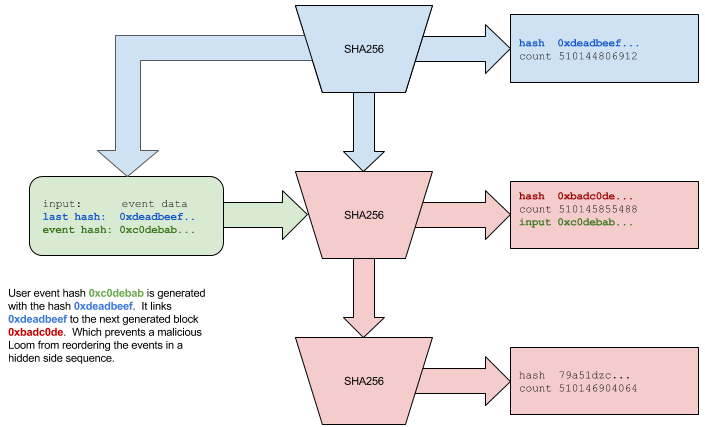
\includegraphics[width=0.9\textwidth]{figures/fig_6.png}
    \caption[Fig 6]{Input con retro riferimento.\label{fig:poh_consistency}}
  \end{center}
  \end{figure}

In Figura~\ref{fig:poh_consistency}, l'input fornito dall'utente dipende dall'hash \texttt{0xdeadbeef\ldots} esistente nella sequenza generata prima che l'hash fosse inserito. La freccia blu in alto a sinistra indica che il client sta facendo riferimento a un hash prodotto in precedenza. Il messaggio del client è valido solo in una sequenza che contiene l'hash \texttt{0xdeadbeef\ldots}. Il colore rosso nella sequenza indica che la sequenza è stata modificata dai dati del client	.

\subsection{Generalità}
4000 hash al secondo genererebbero 160 kilobytes addizionali di dati e avrebbero bisogno di una GPU con 4000 core e circa 0.25-0.75 millisecondi per la verifica.

\subsection{Attacchi}
\subsubsection{Reversal}
 Per generare un ordine inverso è necessario che l'aggressore avvii la sequenza dannosa dopo il secondo evento. Questo ritardo dovrebbe consentire a qualsiasi nodo peer to peer non dannoso di comunicare l'ordine originale.
 
\subsubsection{Velocità}
Avere più generatori può rendere l'implementazione più resistente agli attacchi. Un generatore potrebbe essere ad alta bandwidth 
e potrebbe ricevere molti eventi da mixare nella sua sequenza, un altro generatore potrebbe essere ad alta velocità e bassa bandwidth e potrebbe mescolarsi periodicamente con il generatore di alta larghezza di banda.

La sequenza ad alta velocità creerebbe una sequenza secondaria di dati che un attaccante dovrebbe invertire.

\subsubsection{Attacchi a lungo raggio}

Gli attacchi a lungo raggio comportano l'acquisizione di vecchie chiavi private client dismesse e la generazione di un registro falsificato ~\cite{casper}. La prova storica fornisce una certa protezione contro gli attacchi a lungo raggio. Un utente malintenzionato che ottiene l'accesso a vecchie chiavi private dovrebbe ricreare un record storico che richiede tanto tempo quanto quello originale che sta cercando di falsificare. Ciò richiederebbe l'accesso a un processore più veloce di quello attualmente in uso nella rete, altrimenti l'aggressore non potrebbe mai  raggiungere la lunghezza del record originale! 

Inoltre, un'unica fonte di tempo consente di costruire una prova di riproduzione più semplice (per saperne di più, si veda la Sezione~\ref{porep}). Poiché la rete è progettata in modo che tutti i partecipanti alla rete si basino su un'unica registrazione storica degli eventi.

PoRep e PoH insieme dovrebbero fornire una difesa di spazio e tempo contro un registro falsificato.


\section{Proof of Stake Consensus}\label{proof_of_stake}
\subsection{Descrizione}
Questo esempio specifico di Proof of Stake è progettato per una conferma rapida della sequenza corrente prodotta dal generatore della Proof of History, per votare e selezionare il generatore della Proof of History successivo e per punire qualsiasi validatore che abbia avuto un comportamento scorretto. Questo algoritmo dipende dall'arrivo dei messaggi a tutti i nodi partecipanti entro un certo periodo di tempo.

\subsection{Terminologia}
\begin{description}

\item[bonds]
I bonds sono equivalenti a una spesa in conto capitale nella Proof of Work. Un minatore acquista hardware ed elettricità e li usa in una Blockchain Proof of Work. Il bond è la moneta che il validatore impegna come garanzia durante la convalida delle transazioni.

\item[slashing]

La soluzione proposta al problema della posta in gioco nulla nei sistemi Proof of Stake ~\cite{slasher}. Quando viene pubblicata una prova di voto per un ramo diverso, quel ramo può distruggere il legame del validatore. Si tratta di un incentivo economico volto a scoraggiare i validatori dal confermare più rami.
\item[super maggioranza]
Una super maggioranza è data dai \(\frac{2}{3}\) dei validatori pesati secondi i loro legami. Un voto a super maggioranza indica che la rete ha raggiunto il consenso, e almeno \(\frac{1}{3}\) della rete dovrebbe votare in maniera non onesta per invalidare questo ramo. Il costo economico di un attacco sarebbe quindi pari a \(\frac{1}{3}\) del market cap della moneta.

\end{description}

\subsection{Bonding}
Una transazione di bonding prende una quantità di coin \hyphenation{user specified} e la trasferisce su un conto di bonding con l'identità dell'utente. Le monete nell'account bonding non possono essere spese e devono rimanere nell'account fino a quando l'utente non le rimuove. L'utente può rimuovere solo le monete stantie che sono scadute. Le obbligazioni sono valide dopo che la super maggioranza degli attuali stakeholder ha confermato la sequenza.


\subsection{Voto}
Si prevede che il generatore di Proof of History sarà in grado di pubblicare una firma dello stato in un periodo predefinito. Ogni identità vincolata deve confermare tale firma pubblicando la propria firma dello Stato. La votazione è un semplice sì, senza un no. Se la super maggioranza delle identità vincolate vota entro un timeout, allora questo ramo viene accettato come valido.

\subsection{Unbonding}

Il numero N di voti mancanti marchia i coin come stazionari e non più idonei al voto. L'utente può emettere una transazione di unbonding per rimuoverli.

N è un valore dinamico basato sul rapporto tra voti stazionari e voti attivi. N aumenta all'aumentare del numero di voti stazionari. In caso di partizione di rete di grandi dimensioni, ciò consente un ripristino più rapido del ramo più grande rispetto a quello più piccolo.


\subsection{Elezioni}\label{subsec:elections}
L'elezione di un nuovo generatore di PoH avviene quando viene rilevato un guasto del generatore di PoH. Il validatore con il maggior potere di voto, o il maggior numero di chiavi pubbliche in caso di parità, viene scelto come nuovo generatore di PoH.

Una super maggioranza di conferme è richiesta per la nuova sequenza. Se il nuovo leader fallisce prima che sia disponibile una conferma a maggioranza superiore, viene selezionato il validatore successivo più alto ed è necessaria una nuova serie di conferme.

Per cambiare voto, un validatore deve votare ad un contatore di sequenza PoH più alto, e il nuovo voto deve contenere i voti che vuole cambiare. In caso contrario, la seconda votazione sarà tagliata fuori (slashable vote). La commutazione dei voti dovrebbe essere progettata in modo tale che possa avvenire solo a un'altezza che non abbia una super maggioranza.

Una volta che un generatore di PoH è stabilito è possibile sceglierne uno Secondario per assumere i compiti di elaborazione transazionale. Il Secondario, qualora esistesse, verrebbe scelto come leader se ci fosse un guasto con il Primario.

Se viene rilevata un'eccezione o in base a un programma predefinito la piattaforma fa in modo che il Secondario diventi Primario e i generatori di rango inferiore siano promossi.
\subsection{Election Triggers}
\subsubsection{Fork di un Generatore Proof of History}

I generatori di PoH sono progettati con un'identità che contraddistingue la sequenza generata. Il fork può essere utilizzato solo se l'identità del generatore di PoH è stata compromessa. Viene rilevato un fork perché sono stati pubblicati due diversi record storici sulla stessa identità PoH.

\subsubsection{Eccezioni di Runtime}
Un guasto hardware, un bug o un errore intenzionale nel generatore di PoH potrebbe causare la generazione di uno stato non valido e la pubblicazione di una firma dello stato che non corrisponde al risultato del validatore locale. I validatori pubblicheranno la firma corretta tramite gossip e questo evento innescherebbe un nuovo turno di elezioni.I bond di tutti i validatori che accettano uno stato invalido verranno tagliati (slashed).

\subsubsection{Network Timeouts}

Un network timeout innescherebbe una votazione.

\subsection{Slashing}
Lo slashing si verifica quando un validatore vota due sequenze separate. Una prova di voto malevolo eliminerà i coin dalla circolazione e li aggiungerà alla mining pool.

Una votazione che includa una voto precedente su una sequenza consecutiva non prova una votazione maligna. Anziché tagliare i bond, questa votazione elimina il voto attualmente espresso sulla sequenza delle votazioni in corso.

Si verifica uno slashing anche se si vota per un hash non valido generato dal generatore di PoH. Il generatore dovrebbe generare casualmente uno stato non valido, che innescherebbe un ripiego sul Secondario.
\subsection{Elezioni secondarie}
È possibile proporre e approvare generatori Secondari e di rango inferiore. Una proposta viene lanciata sulla sequenza del generatore primario. La proposta contiene un timeout, se la mozione viene approvata a maggioranza dei voti prima del timeout, il Secondario si considera eletto, e assumerà le funzioni come previsto. Il primario può passare al secondario in maniera delicata inserendo un messaggio nella sequenza generata che indica che si verificherà un passaggio, o inserendo uno stato non valido e costringendo la rete a tornare al secondario.

Se viene eletto un Secondario, e il primario fallisce, il Secondario sarà considerato come il primo ripiego durante le elezioni.


\subsection{Disponibilità}\label{availability}
I sistemi CAP che si occupano di partizioni devono scegliere Coerenza o Disponibilità. Il nostro approccio alla fine sceglie la Disponibilità, ma poiché abbiamo una misura oggettiva del tempo, la Coerenza viene scelta con ragionevoli timeout umani.

I verificatori della Proof of Stake bloccano una certa quantità di coin in una "posta" (stake), il che permette loro di votare per una particolare serie di transazioni. La moneta bloccata è una transazione che viene inserita in un flusso PoH, proprio come qualsiasi altra transazione. Per votare, un verificatore del PoS deve firmare l'hash dello stato che è stato calcolato dopo aver elaborato tutte le transazioni in una posizione specifica nel registro del PoH. Anche questo voto è inserito come transazione nel flusso di PoH. Osservando il registro PoH, possiamo dedurre quanto tempo è trascorso tra una votazione e l'altra e, se si verifica una partizione, per quanto tempo ogni verificatore non è stato disponibile.

Per gestire le partizioni con tempi umani ragionevoli, proponiamo un approccio dinamico ai verificatori non disponibili (unstaking). Quando il numero di verificatori è elevato e superiore a \(\frac{2}{3}\), il processo di "unstaking" può essere veloce. Il numero di hash che devono essere generati nel libro mastro è basso prima che la posta non disponibile dei verificatori venga completamente ignorata e che essi non vengano più presi in considerazione per il consenso. Quando il numero di verificatori è inferiore a \(\frac{2}{3}\)ma superiore a \(\frac{1}{2}\), il timer di rimozione delle stake è più lento e richiede la generazione di un numero maggiore di hash prima che i verificatori mancanti vengano rimossi. In una partizione di grandi dimensioni, come una partizione in cui mancano \(\frac{1}{2}\) o più dei verificatori, il processo di unstaking è molto lento. Le transazioni possono ancora essere inserite nel flusso e i verificatori possono ancora votare, ma il consenso completo di \(\frac{2}{3}\)non sarà raggiunto fino a quando non sarà stata generata una grande quantità di hash e i verificatori non disponibili non saranno stati identificati. La differenza di tempo per riacquistare vitalità da ai client la possibilità di avere tempo per scegliere una partizione che vogliamo continuare a utilizzare.

\subsection{Recupero}\label{availability}
Nel sistema che proponiamo, il libro mastro può essere completamente recuperato da qualsiasi guasto. Ciò significa che chiunque nel mondo può scegliere qualsiasi punto casuale nel libro mastro e creare un fork valido aggiungendo hash e transazioni. Se tutti i verificatori fossero assenti in questo fork, ci vorrebbe molto tempo per far si che qualsiasi bond aggiuntivo diventi valido e  per far raggiungere a questo ramo il consenso della super maggioranza a \(\frac{2}{3}\). Quindi il ripristino completo con zero validatori disponibili richiederebbe un'enorme quantità di hash da aggiungere al libro mastro e i nuovi bond sarebbero in grado di convalidare il libro mastro solo dopo la rimozione di tutti i validatori non disponibili.

\subsection{Finalità}\label{availability}
Il PoH consente ai verificatori della rete di osservare ciò che è accaduto in passato con un certo grado di certezza del momento in cui si sono verificati tali eventi. Poiché il generatore di PoH sta producendo un flusso di messaggi, tutti i verificatori sono tenuti a inviare le loro firme dello stato entro 500ms. Questo numero può essere ulteriormente ridotto in base alle condizioni di rete. Poiché ogni verifica viene inserita nel flusso, tutti in rete possono validare che ogni verificatore ha inviato il proprio voto entro il tempo richiesto senza osservare direttamente il voto.

\subsection{Attacchi}
\subsubsection{Tragedia dei beni comuni}
I verificatori PoS confermano semplicemente l'hash di stato generato dal generatore PoH. C'è un incentivo economico per loro a non fare alcun lavoro e approvare semplicemente  ogni stato generato dall'hash . Per evitare questa condizione, il generatore di PoH dovrebbe immettere un hash non valido a intervalli casuali. Tutti i votanti questo hash dovrebbero essere tagliati fuori (slashed). Quando l'hash viene generato, la rete dovrebbe promuovere immediatamente il generatore di PoH Secondario eletto.

Ogni verificatore è tenuto a rispondere entro un breve periodo di tempo, ad esempio 500 ms. Il timeout dovrebbe essere impostato a un livello sufficientemente basso da far sì che un verificatore malintenzionato abbia una bassa probabilità di osservare un altro voto dei verificatori e di introdurre i propri voti nel flusso con velocità sufficiente.


\subsubsection{Collusione con il lgeneratore PoH}\label{subsubsec:collusion}
Un verificatore in collusione con il generatore di PoH saprebbe in grado di prevedere quando verrà prodotto l'hash non valido e non voterebbe a favore. In realtà, questo scenario non è diverso dall'identità del PoH con una quota di partecipazione (stake) più ampia da parte del verificatore. Il generatore di PoH deve ancora fare tutto il lavoro necessario per produrre l'hash di stato.

\subsubsection{Censura}\label{censorship}
La censura o il rifiuto del servizio potrebbero verificarsi quando un \(\frac{1}{3}\) dei possessori di bond rifiuta di convalidare qualsiasi sequenza con nuove obbligazioni. Il protocollo può difendersi da questa forma di attacco regolando dinamicamente la velocità con cui i legami diventano statici. In caso di rifiuto del servizio, la partizione più grande sarà progettata per forzare e censurare i titolari di bond bizantini (Byzantine bond holders). La rete più grande si ripristinerà grazie ai Byzantine bond che diventano statici . La partizione bizantina più piccola non è in grado di andare avanti per un periodo di tempo più lungo.

L'algoritmo funziona come segue. La maggioranza della rete eleggerebbe un nuovo leader. Il Leader censurerebbe i detentori di bond bizantini e non li farebbe partecipare. Il generatore di Proof of History dovrebbe continuare a generare una sequenza, per dimostrare il passare del tempo, fino a quando abbastanza Byzantine bond non diventino staticiin modo da ottenere una super maggioranza nella rete più grande. Il tasso con cui i bond diventano statici verrebbe basato dinamicamente su quae percentuale di bond è attiva. Così il fork bizantino di minoranza della rete dovrebbe aspettare molto più a lungo della di quello di maggioranza per recuperare una super maggioranza. Una volta che è stata stabilita una super maggioranza, lo slashing potrebbe essere usato per punire in modo permanente i detentori di bond bizantini.

\subsubsection{Attacchi a lungo raggio}\label{censorship}
PoH fornisce una difesa naturale contro gli attacchi a lungo raggio. Recuperare il registro da qualsiasi punto del passato richiederebbe all'attaccante di superare il registro valido superando la velocità del generatore di PoH.

Il protocollo di consenso fornisce un secondo livello di difesa, in quanto qualsiasi attacco richiederebbe più tempo di quello necessario per rimuovere tutti i validatori validi. Crea anche un "gap" di disponibilità nella storia del libro mastro. Confrontando due libri contabili della stessa altezza, si può oggettivamente considerare valido quello con la più piccola massima partizione.

\subsubsection{Attacchi ASIC}\label{censorship}

In questo protocollo esistono due opportunità per gli attacchi ASIC: durante la partizione e con timeout fasulli durante la Finalità.

Per gli attacchi ASIC durante le partizioni, la velocità con la quale i bond sono tolti dallo stake non è lineare, e per le reti con partizioni di grandi dimensioni la velocità è inferiore agli ordini di grandezza dei guadagni attesi da un attacco ASIC.

Per gli attacchi ASIC durante la Finalità, la vulnerabilità permette ai validatori bizantini che hanno un bond in gioco (bonded stake) di aspettare conferme da altri nodi e di immettere i loro voti con un generatore di PoH collaborante. Il generatore PoH può quindi utilizzare il suo ASIC più veloce per generare 500 ms di hash in meno tempo e consentire la comunicazione di rete tra il generatore PoH e i nodi collaboranti. Ma, se il generatore di PoH è anche bizantino, non c'è ragione per cui debba comunicare il contatore esatto quando si prevede di inserire il guasto. Questo scenario non è diverso da quello in cui un generatore di PoH e tutti i collaboratori condividono la stessa identità e quando hanno un unico stake combinato e usano solo 1 set di hardware.

\section{Prova di Replicazione in Streaming}\label{porep}
\subsection{Descrizione}
Filecoin ha proposto una versione della Proof of Replication \cite{filecoinporep}. L'obiettivo di questa versione è quello di avere verifiche rapide e in streaming della Proof of Replication, che sono abilitate tenendo traccia del tempo in una sequenza generata dalla Proof of History. La replica non è usata come un algoritmo di consenso, ma è uno strumento utile per tenere conto del costo di memorizzazione della cronologia della Blockchain o dello stato ad alta disponibilità.
\subsection{Algoritmo}
Come mostrato in Figura~\ref{fig:encrypt} la crittografia CBC crittografa ogni blocco di dati in sequenza, utilizzando il blocco precedentemente crittografato per XOR i dati di input.

\begin{figure}[h]
  \begin{center}
    \centering
    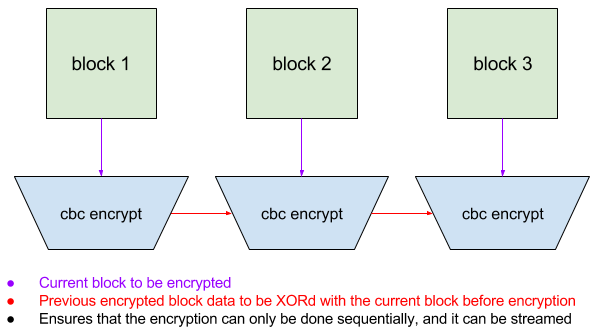
\includegraphics[width=0.9\textwidth]{figures/cbc_encryption_001.png}
    \caption[Fig 7]{Crittografia sequenziale CBC\label{fig:encrypt}}
  \end{center}
  \end{figure}

Ogni copia dell'identità genera una chiave firmando un hash creato tramite una sequenza ddella Proof of History. Ciò lega la chiave all'identità del replicatore e a una specifica sequenza di Proof of Work. È possibile selezionare solo hash specifici. (Vedere Sezione ~\ref{hashselection} sulla selezione del hash)

Il set di dati è completamente crittografato blocco per blocco. Quindi, per generare una prova, la chiave viene utilizzata per avviare un generatore di numeri pseudo casuali che seleziona un numero casuale di 32 byte da ogni blocco.

Viene calcolato un hash di merkle con l'hash della PoH aggiunto a ciascuna sezione.

\begin{figure}[h]
  \begin{center}
    \centering
    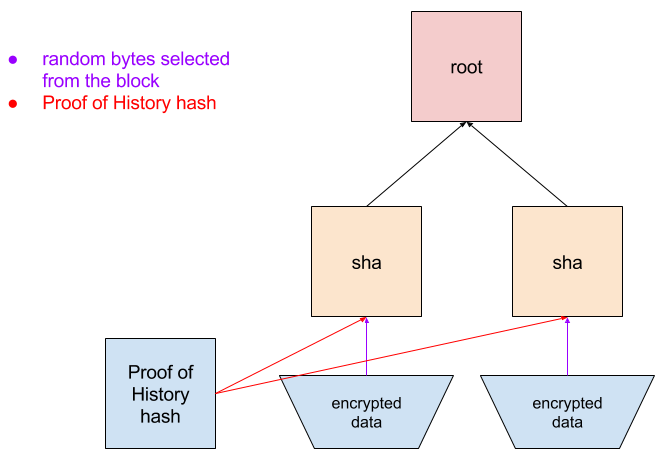
\includegraphics[width=0.9\textwidth]{figures/por_001.png}
    \caption[Fig 8]{Fast Proof of Replication\label{fig_8}}
  \end{center}
  \end{figure}

La root viene pubblicata insieme alla chiave e all'hash selezionato che è stato generato. Il nodo di replica è necessario per pubblicare un'altra prova in N hash mentre vengono generati dal generatore della Proof of History, dove N è circa \(\frac{1}{2}\) il tempo necessario per crittografare i dati. Il generatore della Proof of History pubblicherà hash specifici per la Proof of replication a periodi predefiniti. Il nodo replicatore deve selezionare l'hash successivo pubblicato per generare la prova. Anche in questo caso, l'hash viene firmato e vengono selezionate delle porzioni casuali dai blocchi per creare la radice di merkle.

Dopo un periodoN prove, i dati vengono nuovamente crittografati con una nuova chiave CBC.
\subsection{Verifica}

Con N core, ogni core è in grado di eseguire lo streaming crittografico per ogni identità. Lo spazio totale richiesto è \(2 blocchi * N cores\), dal momento che il precedente blocco cifrato è necessario per generare il successivo. Ciascun nucleo può quindi essere utilizzato per generare tutte le prove che sono state derivate dal blocco crittografato corrente.

Il tempo totale necessario per verificare le prove di stampa dovrebbe essere pari al tempo necessario per la crittografia. Le prove stesse consumano pochi byte casuali dal blocco, quindi la quantità di dati in hash è significativamente inferiore alla dimensione del blocco crittografato. Il numero di identità di replica verificabili contemporaneamente è uguale al numero di core disponibili. Le GPU moderne hanno a disposizione oltre 3500 core, anche se a \(\frac{1}{2}\)-\(\frac{1}{3}\) della velocità di clock di una CPU.

\subsection{Rotazione delle chiavi}

Senza rotazione delle chiavi, la stessa replica crittografata può generare prove per più sequenze di Proof of History. Le chiavi vengono ruotate periodicamente e ogni replica viene ricrittografata con una nuova chiave legata a una sequenza unica di Proof of History.

La rotazione deve essere abbastanza lenta da rendere pratica la verifica delle prove di replica sull'hardware della GPU, che è più lenta per core rispetto alle CPU.

\subsection{Selezione degli Hash}\label{hashselection}

Il generatore Proof of History pubblica un hash che deve essere utilizzato dall'intera rete per crittografare le Proofs of Replication e per utilizzarlo come generatore di numeri psudo casuali per la selezione dei byte nelle prove rapide.

L'hash è pubblicato su un contatore periodico che è approssimativamente uguale a \(\frac{1}{2}\) il tempo necessario per crittografare il set di dati. Ogni identità di replica deve usare lo stesso hash e usare il risultato firmato dell'hash come seed per la selezione dei byte, o la chiave di crittografia.

Il periodo che ogni replicatore deve fornire per la prova deve essere inferiore al tempo di crittografia. In caso contrario, il replicatore può eseguire lo streaming della crittografia ed eliminarla per ogni prova.

Un generatore dannoso potrebbe immettere dati nella sequenza prima di questo hash per generare un hash specifico. Questo attacco è discusso più approfonditamente su \ref{subsubsec:collusion}.

\subsection{Convalida della prova}
Il nodo della Proof of History non è tenuto a convalidare le Proofs of replication presentate. Essa dovrebbe tenere traccia del numero di prove in sospeso e verificate che vengono fornite dall'identità del replicatore. Una prova deve essere verificata quando il replicatore è in grado di firmarla da una super maggioranza dei validatori della rete.

Le verifiche sono raccolte dal replicatore tramite p2p gossip network, e presentate come un pacchetto che contiene una super maggioranza dei validatori in rete. Questo pacchetto verifica tutte le prove prima di uno specifico hash generato dalla sequenza Proof of History e può contenere più identità di replicatori contemporaneamente.
\subsection{Attacchi}
\subsubsection{Spam}
Un utente malintenzionato potrebbe creare molte identità di replicatore e spamare la rete con prova false. Per facilitare una verifica più rapida, i nodi sono tenuti a fornire i dati crittografati e l'intero albero di merkle al resto della rete quando richiedono la verifica.

La Proof of Replication che è progettata in questo documento consente una verifica economica di qualsiasi prova aggiuntiva, in quanto non richiede spazio aggiuntivo. Ma ogni identità richiederebbe 1 nucleo di tempo di crittografia. L'obiettivo di replica dovrebbe essere fissato ad una dimensione massima dei core facilmente disponibili. Le GPU moderne sono dotate di oltre 3500 core.

\subsubsection{Cancellazione Parziale}

Un nodo del replicatore potrebbe tentare di cancellare parzialmente alcuni dati per evitare di memorizzare l'intero stato. Il numero di prove e la casualità del seme dovrebbe rendere difficile questo attacco.

Ad esempio, un utente che memorizza 1 terabyte di dati cancella un singolo byte da ogni blocco di 1 megabyte. Un'unica prova che campiona 1 byte su ogni megabyte avrebbero una probabilità di collisione con qualsiasi byte cancellato pari a \(1 - (1- 1/1.000.0000)^{1.000.000} = 0,63\). Dopo 5 prove la probabilità è \(0.99\).

\subsubsection{Collusione con il generatore di Proof of History}

Si prevede di utilizzare l'hash firmato per preparare il campione. Se un replicatore è in grado di selezionare in anticipo un hash specifico, può cancellare tutti i byte che non vengono campionati.

Un'identità di replicatore collusiva con il generatore della Proof of History potrebbe immettere una transazione specifica alla fine della sequenza prima che venga generato l'hash predefinito per la selezione casuale dei byte. Con un numero sufficiente di core, un attaccante potrebbe generare un hash preferibile all'identità del replicatore.

Questo attacco potrebbe andare a vantaggio di un'unica identità di replicatore. Poiché tutte le identità devono utilizzare lo stesso hash esatto che è crittograficamente firmato con ECDSA (o equivalente), la firma risultante è unica per ogni identità del replicatore ed è resistente alle collisioni. Un'unica identità di replicatore avrebbe solo vantaggi marginali.
\subsubsection{Rifiuto del Servizio}
Il costo dell'aggiunta di un'identità di replicatore aggiuntiva dovrebbe essere pari al costo dello storage. Il costo dell'aggiunta di capacità di calcolo aggiuntive per verificare tutte le identità del replicatore dovrebbe essere pari al costo di una CPU o di un nucleo di GPU per identità di replica.

Ciò crea l'opportunità di un attacco di rifiuto del servizio alla rete creando un gran numero di identità di replicatori valide.

Per limitare questo attacco, il protocollo di consenso scelto per la rete può selezionare un target di replica e assegnare le prove di replica che soddisfano le caratteristiche desiderate, come la disponibilità sulla rete, la larghezza di banda, la geolocalizzazione, ecc ...
\subsubsection{Tragedia dei Beni Comuni}

	I verificatori PoS possono semplicemente confermare la PoRep senza fare alcun lavoro. Gli incentivi economici dovrebbero essere messi in relazione con i verificatori del PoS per svolgere il loro lavoro, vale a dire suddividere il pagamento del mining tra i verificatori del PdS e i nodi di replicazione del PoRep.
	
	Per evitare ulteriormente questo scenario, i verificatori PoRep possono presentare prove false per piccoli periodi. Possono dimostrare che la prova è falsa fornendo la funzione che ha generato i dati falsi. Qualsiasi verificatore del PoS che avesse confermato una falsa prova sarebbe stato tagliato fuori (slashed).
	
\section{Architettura di Sistema}\label{system_architecture}

\begin{figure}
  \begin{center}
    \centering
    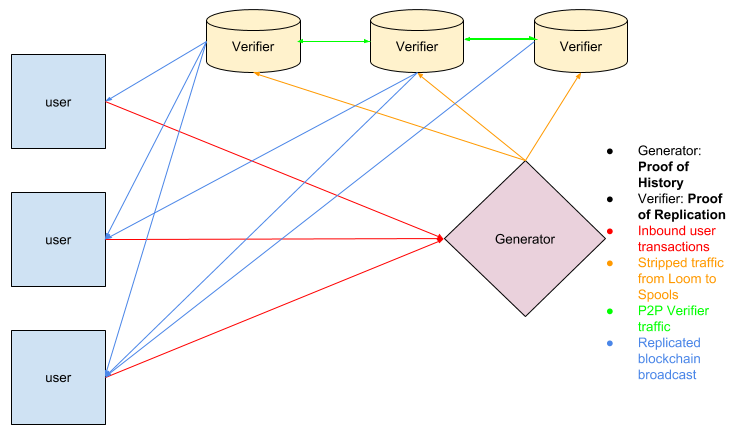
\includegraphics[width=0.9\textwidth]{figures/system_arch_001.png}
    \caption[Fig 9]{Architettura di Sistema \label{fig_9}}
  \end{center}
  \end{figure}

\subsection{Componenti}

\subsubsection{Leader, Generatore Proof of History}
Il Leader è un generatore eletto della Proof of History. Utilizza transazioni arbitrarie degli utenti e produce una sequenza della Proof of History di tutte le transazioni che garantiscono un ordine globale unico nel sistema. Dopo ogni batch di transazioni il Leader emette una firma dello stato che è il risultato dell'esecuzione delle transazioni in quell'ordine. Tale firma è fatta con l'identità del Leader.

\subsubsection{Stato}
Lo stato è una tabella hash non univoca indicizzata in base all'indirizzo dell'utente. Ogni cella contiene l'indirizzo completo dell'utente e la memoria necessaria per questo calcolo. 	Ad esempio,\\
\noindent la tabella delle transazioni contiene:\\\\\noindent
\begin{bytefield}[bitwidth=.1em]{256}
\bitheader{0,31,63,95,127,159,191,223,255} \\
\bitbox{160}{Ripemd delle Public Key  Utenti}
& \bitbox{64}{Account}
& \bitbox{32}{unused}
\end{bytefield}\\
per un totale di 32 bytes.\\
\noindent La tabella dei bond della Proof of Stake contiene:\\\\\noindent
\begin{bytefield}[bitwidth=.1em]{256}
\bitheader{0,31,63,95,127,159,191,223,255} \\
\bitbox{160}{Ripemd delle Public Key  Utenti}
& \bitbox{64}{Bond} \\
& \bitbox{64}{Ultimo voto} \\
& \bitbox{224}{unused}
\end{bytefield}\\
per un totale di 64 bytes.
\subsubsection{Verificatore, Replicazione di stato}



I nodi di verifica si replicano e garantiscono un'elevata disponibilità dello stato della Blockchain. L'obiettivo di replica è selezionato dall'algoritmo di consenso e i validatori nell'algoritmo di consenso selezionano e votano i nodi della Proof of Replication che approvano sulla base di criteri definiti fuori catena.


La rete può essere configurata con una dimensione minima del bond della Proof of Stake e il requisito di un'unica identità di replicatore per bond.
\subsubsection{Validatori}
Questi nodi occupano la larghezza di banda dei Verificatori. Sono nodi virtuali e possono essere eseguiti sulle stesse macchine dei verificatori o del leader, oppure su macchine separate  specifiche per l'algoritmo di consenso configurato per questa rete.


\subsection{Limiti di Rete}

\begin{figure}
  \begin{center}
    \centering
    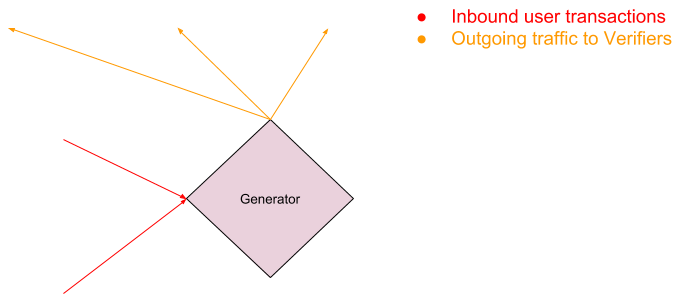
\includegraphics[width=0.8\textwidth]{figures/generator_network_limits_001.png}
    \caption[Fig 10]{Limiti di rete del Generatore \label{fig_10}}
  \end{center}
  \end{figure}

Il leader deve essere in grado di prendere i pacchetti di utenti in arrivo, ordinarli nel modo più efficiente possibile e sequenziarli in una lista della Proof of History pubblicata sui verificatori a valle. L'efficienza è basata su modelli di accesso alla memoria delle transazioni, in modo che le transazioni siano ordinate per ridurre al minimo i guasti e massimizzare il prefetching.\\\\

\noindent \textbf{Formato dei pacchetti in entrata:}\\\\\noindent
\begin{bytefield}[bitwidth=.1em]{256}
\bitheader{0,31,63,95,127,159,191,223,255} \\
\begin{rightwordgroup}{Firmato}
\bitbox{160}{Ultimo Hash Valido}
& \bitbox{64}{Contatore}
& \bitbox{6}{u}
& \bitbox{10}{s} \\
& \bitbox{64}{Commisioni} \\
& \bitbox{256}{Da} \\
\end{rightwordgroup} \\
& \bitbox{256}{Firma 1 di 2} \\
& \bitbox{256}{Firma 2 di 2} \\
\end{bytefield}

\noindent Dimensione \(20 + 8 + 16 + 8 + 32 + 32 + 32 = 148\) bytes.\\\\

Il payload minimo che può essere supportato è 1 account di destinazione con una dimensione minima di 176 byte.\\\\

\noindent \textbf{Con payload:}\\\\\noindent

\begin{bytefield}[bitwidth=.1em]{256}
\bitheader{0,31,63,95,127,159,191,223,255} \\
\begin{rightwordgroup}{Firmato}
\bitbox{160}{Ultimo Hash Valido}
& \bitbox{64}{Contatore}
& \bitbox{6}{u}
& \bitbox{10}{s} \\
& \bitbox{160}{A}
& \bitbox{64}{Ammontare} \\
& \bitbox{64}{Contatore}
& \bitbox{64}{Commissioni} \\
& \bitbox{256}{Da} \\
\end{rightwordgroup} \\
& \bitbox{256}{Firma 1 di 2} \\
& \bitbox{256}{Firma 2 di 2} \\
\end{bytefield}

\noindent Con dimensione minima del payload pari a: 176 bytes\\\\

Il pacchetto della sequenza Proof of History contiene l'hash corrente, il contatore e l'hash di tutti i nuovi messaggi aggiunti alla sequenza PoH e la firma di stato dopo l'elaborazione di tutti i messaggi. Questo pacchetto viene inviato ogni volta che vengono trasmessi N messaggi .\\
\noindent Pacchetti Proof of History:\\\\\noindent
\begin{bytefield}[bitwidth=.1em]{256}
\bitheader{0,31,63,95,127,159,191,223,255} \\
\begin{rightwordgroup}{Firmato}
\bitbox{160}{Hash Corrente}
& \bitbox{64}{Contatore} \\
\bitbox{160}{Hash Messaggi} \\
\bitbox{160}{Hash Stato} \\
\end{rightwordgroup} \\
& \bitbox{256}{Firma 1 di 2} \\
& \bitbox{256}{Firma 2 di 2} \\
\end{bytefield}

\noindent La dimensione minima del pacchetto in uscita è : 132 bytes \\\\

Su una connessione di rete a 1 gbps il numero massimo di transazioni possibili è $1$~gigabit al secondo / $176$~bytes = $710$k tps max. Si prevede una certa perdita ($1-4\%$) a causa del framing Ethernet. La capacità inutilizzata che supera la quantità prevista per la rete può essere utilizzata per aumentare la disponibilità codificando l'output con i codici Reed-Solomon e rimuovendolo dai Verificatori a valle disponibili.
\subsection{Limiti Computazionali}
Ogni transazione richiede una verifica del contenuto di un compendio. Questa operazione non utilizza alcuna memoria al di fuori del messaggio di transazione stesso e può essere effettuata in parallelo in modo indipendente. La produttività dovrebbe quindi essere limitata dal numero di core disponibili sul sistema.

I server di verifica ECDSA basati su GPU hanno avuto risultati sperimentali di operazioni 900k al secondo~\cite{gpuecc}.
\subsection{Limiti di Memoria}
Un'implementazione grezza dello stato come un \(50\%\) hashtable completo con 32 byte di voci per ogni account, sarebbe teoricamente in grado di mettere 10 miliardi di conti in 640GB. L'accesso casuale allo stato stabile a questa tabella è misurato su \(1.1 * 10^7\) scritture o letture al secondo. Sulla base di 2 letture e 2 scritture per transazione, il throughput di memoria è in grado di gestire 2,75 milioni di transazioni al secondo. Questo è stato misurato su un'istanza di Amazon Web Services da 1 TB x 1,16x.

\subsection{Smart Contracts ad alte Performance}\label{sec:smartcontracts}

Gli Smart Contract sono una forma generalizzata di transazioni, programmi che girano su ogni nodo e modificano lo stato. Questo design sfrutta il bytecode esteso Berkeley Packet Filter, veloce e facile da analizzare e il bytecode JIT come linguaggio per i contratti intelligenti.

Uno dei suoi principali vantaggi è un'interfaccia a costo zero per funzioni esterne. Le funzioni intrinseche o di alto livello implementate direttamente sulla piattaforma sono richiamabili dai programmi forniti dall'utente. Chiamare l'intrinseco sospende il programma e pianifica l'intrinseco su un server ad alte prestazioni. Gli intrinseci sono raggruppati per eseguire l'esecuzione in parallelo sulla GPU.
\begin{figure}
  \begin{center}
    \centering
    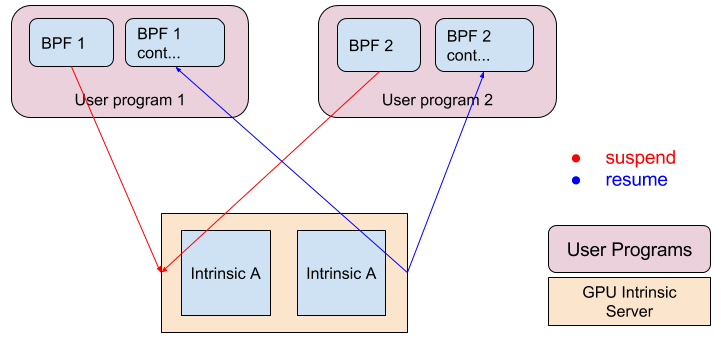
\includegraphics[width=0.9\textwidth]{figures/bpf_programs_001.png}
    \caption[Fig 11]{Esecuzione dei programmi BPF definiti dall'utente.\label{fig_11}}
  \end{center}
  \end{figure}

Nell'esempio precedente, due diversi programmi utente chiamano lo stesso intrinseco. Ogni programma viene sospeso fino al completamento dell'esecuzione batch degli elementi intrinseci. Un esempio intrinseco è la verifica dell'ECDSA. Il confronto di queste chiamate per l'esecuzione sulla GPU può aumentare il throughput di migliaia di volte.

Questo trampolino non richiede interruttori di contesto del thread nativi del sistema operativo, poiché il bytecode BPF ha un contesto ben definito per tutta la memoria che sta utilizzando.

Il back end eBPF è stato incluso nell'LLVM dal 2015, quindi qualsiasi linguaggio di frontend dell'LLVM può essere usato per scrivere Smart Contract. È nel kernel Linux dal 2015 e le prime iterazioni del bytecode sono in circolazione dal 1992. Un singolo passaggio può controllare la correttezza dell'eBPF, accertarne il tempo di esecuzione e i requisiti di memoria e convertirlo in istruzioni x86.

\bibliographystyle{abbrv}
\bibliography{simple}

\begin{thebibliography}{9}
\bibitem{liskov}
Liskov, Practical use of Clocks
\\\texttt{ http://www.dainf.cefetpr.br/~tacla/SDII/PracticalUseOfClocks.pdf}

\bibitem{spanner}
Google Spanner TrueTime consistency
\\\texttt{ https://cloud.google.com/spanner/docs/true-time-external-consistency}

\bibitem{ordering}
Solving Agreement with Ordering Oracles
\\\texttt{ http://www.inf.usi.ch/faculty/pedone/Paper/2002/2002EDCCb.pdf}

\bibitem{tendermint}
Tendermint: Consensus without Mining
\\\texttt{https://tendermint.com/static/docs/tendermint.pdf}

\bibitem{hashgraph}
Hedera: A Governing Council \& Public Hashgraph Network
\\\texttt{https://s3.amazonaws.com/hedera-hashgraph/hh-whitepaper-v1.0-180313.pdf}

\bibitem{filecoinporep}
Filecoin, proof of replication,
\\\texttt{https://filecoin.io/proof-of-replication.pdf}

\bibitem{slasher}
Slasher, A punative Proof of Stake algorithm
\\\texttt{https://blog.ethereum.org/2014/01/15/slasher-a-punitive-proof-of-stake-algorithm/}

\bibitem{delegatedpos}
BitShares Delegated Proof of Stake
\\\texttt{https://github.com/BitShares/bitshares/wiki/Delegated-Proof-of-Stake}

\bibitem{gpuecc}
An Efficient Elliptic Curve Cryptography Signature Server With GPU Acceleration
\\\texttt{http://ieeexplore.ieee.org/document/7555336/}

\bibitem{casper}
Casper the Friendly Finality Gadget
\\\texttt{https://arxiv.org/pdf/1710.09437.pdf}
\end{thebibliography}
\end{document}
This is never printed
